\documentclass[11pt,a4paper,oneside]{article}

%%%%%%%%%%%%%%%%%%%%%%%%%%%%%%%%%%%%%%%%%%%%%%%%%%%%%%%%%%%%%%%%%%%%%%%%%%%%%%%%
% Packages
%%%%%%%%%%%%%%%%%%%%%%%%%%%%%%%%%%%%%%%%%%%%%%%%%%%%%%%%%%%%%%%%%%%%%%%%%%%%%%%%

% Fonts
\usepackage{fontspec}
\setmainfont{Times New Roman}

% Language
\usepackage[british, greek]{babel}

% Unicode
\usepackage{xunicode}
\usepackage[utf8x]{inputenc}

% Links
\usepackage{hyperref}

% Algorithms
\usepackage{algorithm}
\usepackage{algpseudocode}

% Ceil
\usepackage{mathtools}
\DeclarePairedDelimiter{\ceil}{\lceil}{\rceil}

% Graphics
\usepackage{graphicx}
\graphicspath{{graphs/}}

% Margin
\usepackage[margin=2cm]{geometry}

% Code formatting
\usepackage{minted}
\newminted{console}{numbersep=5pt,frame=lines,framesep=2mm,gobble=4,fontsize=\footnotesize}

%%%%%%%%%%%%%%%%%%%%%%%%%%%%%%%%%%%%%%%%%%%%%%%%%%%%%%%%%%%%%%%%%%%%%%%%%%%%%%%%

\begin{document}

%%%%%%%%%%%%%%%%%%%%%%%%%%%%%%%%%%%%%%%%%%%%%%%%%%%%%%%%%%%%%%%%%%%%%%%%%%%%%%%%
% Metadata
%%%%%%%%%%%%%%%%%%%%%%%%%%%%%%%%%%%%%%%%%%%%%%%%%%%%%%%%%%%%%%%%%%%%%%%%%%%%%%%%

\title{
    {\large Παράλληλα συστήματα}\\
    Εργασία MPI 2014-15:\\
    Συνέλιξη Εικόνων
}
\author{
    \textsc{Γεώργιος Λεστάρης}\\
    (1115-2008-00073)\\
    \href{mailto:g.lestaris@di.uoa.gr}{\texttt{g.lestaris@di.uoa.gr}}
}

%%%%%%%%%%%%%%%%%%%%%%%%%%%%%%%%%%%%%%%%%%%%%%%%%%%%%%%%%%%%%%%%%%%%%%%%%%%%%%%%

%%%%%%%%%%%%%%%%%%%%%%%%%%%%%%%%%%%%%%%%%%%%%%%%%%%%%%%%%%%%%%%%%%%%%%%%%%%%%%%%
% Title
%%%%%%%%%%%%%%%%%%%%%%%%%%%%%%%%%%%%%%%%%%%%%%%%%%%%%%%%%%%%%%%%%%%%%%%%%%%%%%%%

\makeatletter
\begin{center}
    {\LARGE\@title}
\end{center}
\vspace{10pt}
\begin{flushright}
    {\large\@author}
    \\\@date
\end{flushright}
\vspace{20pt}

%%%%%%%%%%%%%%%%%%%%%%%%%%%%%%%%%%%%%%%%%%%%%%%%%%%%%%%%%%%%%%%%%%%%%%%%%%%%%%%%

%%%%%%%%%%%%%%%%%%%%%%%%%%%%%%%%%%%%%%%%%%%%%%%%%%%%%%%%%%%%%%%%%%%%%%%%%%%%%%%%
% Table of contents
%%%%%%%%%%%%%%%%%%%%%%%%%%%%%%%%%%%%%%%%%%%%%%%%%%%%%%%%%%%%%%%%%%%%%%%%%%%%%%%%

\tableofcontents

%%%%%%%%%%%%%%%%%%%%%%%%%%%%%%%%%%%%%%%%%%%%%%%%%%%%%%%%%%%%%%%%%%%%%%%%%%%%%%%%

%%%%%%%%%%%%%%%%%%%%%%%%%%%%%%%%%%%%%%%%%%%%%%%%%%%%%%%%%%%%%%%%%%%%%%%%%%%%%%%%
% Introduction
%%%%%%%%%%%%%%%%%%%%%%%%%%%%%%%%%%%%%%%%%%%%%%%%%%%%%%%%%%%%%%%%%%%%%%%%%%%%%%%%

\section{Introduction}

This document comes along with the image convolution MPI program, developed for
the Parallel systems UoA course. The source code that comes along with this
document contain the parallel implementation of image convolution with MPI,
the serial implementation of image convolution (for reference) and some tests
for the modules (unit tests).

%%%%%%%%%%%%%%%%%%%%%%%%%%%%%%%%%%%%%%%%%%%%%%%%%%%%%%%%%%%%%%%%%%%%%%%%%%%%%%%%

%%%%%%%%%%%%%%%%%%%%%%%%%%%%%%%%%%%%%%%%%%%%%%%%%%%%%%%%%%%%%%%%%%%%%%%%%%%%%%%%
% Structure of the project and communication
%%%%%%%%%%%%%%%%%%%%%%%%%%%%%%%%%%%%%%%%%%%%%%%%%%%%%%%%%%%%%%%%%%%%%%%%%%%%%%%%

\section{Structure of the project and communication}

\begin{algorithm}
\caption{Root process code ($Rank = 0$)}
\begin{algorithmic}[1]
\State $InImg \gets$ Parsed image from RAW file
\Comment{Read files}
\State $Filter \gets$ Parsed filter (matrix) from file
\State \Call{Broadcast}{Filter}
\Comment{Broadcast the filter (collective communication)}
\State $RowIdx \gets 0$
\Comment{Slice and distribute the image (point-to-point communication)}
\State $Limit \gets \ceil[\bigg]{\frac{InImg.Height}{Size - 1}}$
\ForAll{$i \in [1, Size - 1]$}
    \State \Call{SendImgFragment}{$InImg[RowIdx:RowIdx + Limit]$, $i$}
    \State $RowIdx \gets RowIdx + Limit$
\EndFor
\State $RowIdx \gets 0$
\Comment{Collect results (point-to-point communication)}
\ForAll{$i \in [1, Size - 1]$}
    \State \Call{RecvImgFragment}{$OutImg[RowIdx:RowIdx + Limit]$, $i$}
    \State $RowIdx \gets RowIdx + Limit$
\EndFor
\State $OutImg \rightarrow$ Write image to RAW file
\Comment{Write results}
\end{algorithmic}
\end{algorithm}

The \texttt{imcon} program is based on the MPI library for distributed-memory
parallel application development. It uses both the principles of point-to-point
communication and collective communication. There are two types of processes.
A single root process and multiple worker processes.

\subsection{Processes}

The root process takes care of the I/O operations. It reads and parses files
(image and filter) as well as writes the output image to the file system. It
distributes the filter and the image to the worker process and it gathers the
convolution results. To balance the workload through the workers, it slices
the image by height into equally sized parts. Each part is then sent to a
worker process.

The worker process receives the filter and an image part. It runs the
convolution algorithm and sends back the results.

\begin{algorithm}
\caption{Worker process code ($Rank \ne 0$)}
\begin{algorithmic}[1]
\State $Filter \gets$ Broadcasted filter
\Comment{Receives filter}
\State $InImg \gets$ Empty image
\Comment{Receive the input image}
\State $Limit \gets \ceil[\bigg]{\frac{InImg.Height}{Size - 1}}$
\State $RowIdx \gets Rank * Limit$
\State \Call{RecvImgFragment}{$InImg[RowIdx:RowIdx + Limit]$, 0}
\State \Call{ConvolutionPartialRun}{$InImg[RowIdx:RowIdx + Limit]$, $OutImg$}
\Comment{Run convolution}
\State \Call{SendImgFragment}{$OutImg[RowIdx:RowIdx + Limit]$, 0}
\Comment{Send results back}
\end{algorithmic}
\end{algorithm}

\subsection{MPI communication}

The filter distribution is done with \texttt{MPI\_Bcast} method using
collective communication. The input and output image fragment sends and
receives are done with the \texttt{MPI\_Send} and \texttt{MPI\_Recv} methods of
point-to-point communication. Sending just the related fragment of the image to
a worker saves communication resources instead of broadcasting the whole image
to all the workers. The same applies for the transferring of the results.

%%%%%%%%%%%%%%%%%%%%%%%%%%%%%%%%%%%%%%%%%%%%%%%%%%%%%%%%%%%%%%%%%%%%%%%%%%%%%%%%

%%%%%%%%%%%%%%%%%%%%%%%%%%%%%%%%%%%%%%%%%%%%%%%%%%%%%%%%%%%%%%%%%%%%%%%%%%%%%%%%
% Implementation
%%%%%%%%%%%%%%%%%%%%%%%%%%%%%%%%%%%%%%%%%%%%%%%%%%%%%%%%%%%%%%%%%%%%%%%%%%%%%%%%

\section{Implementation}

The code has the following requirements to be compiled and run:

\begin{itemize}
    \item CMake: cross-platform, open-source build system
        (\url{http://www.cmake.org/}).
    \item MPI: an MPI library implementation. Tests were done with Open MPI
        (\url{http://www.open-mpi.org/}).
    \item C Compiler: For the tests Clang was used (Platform was Apple Darwin
        (UNIX)).
\end{itemize}

\subsection{Compilation}

Following commands can be used to compile the project:

\begin{consolecode}
    > cd build/
    > cmake ...
    -- The C compiler identification is AppleClang 6.0.0.6000056
    ...
    -- Generating done
    -- Build files have been written to: /Users/george/di_dev/ParSys/build
    > make
    Scanning dependencies of target ictypes
    [  7%] Building C object CMakeFiles/ictypes.dir/src/lib/types/matrix.c.o
    [ 14%] Building C object CMakeFiles/ictypes.dir/src/lib/types/image.c.o
    ...
    Linking C executable test-types
    [100%] Built target test-types
\end{consolecode}

\subsection{Usage}

The executable is \texttt{imcon}, and it supports the following flags and
options:

\begin{description}
    \item[-d] Input image file path.
    \item[-o] Output image file path.
    \item[-m] Filter matrix file path.
    \item[-y] Image height (in px).
    \item[-x] Image width (in px)
    \item[-s] Image pixel size (in bytes). Optional, default: 1.
    \item[-v] Increases console output verbosity.
    \item[-h] Prints a help message that describes flags and options.
\end{description}

The same interface is supported by the serial convolution implementation:
\texttt{imcon-serial}. The image files are expected to be in the RAW format,
used for the assignment example images. The matrix files look like the
following:

\begin{consolecode}
    > cat ../test_datasets/in/sharpen.txt
    -2 -1 0
    -1 1 1
    0 1 2
\end{consolecode}

The process normally does not print messages, unless the verbosity is increased
(the \texttt{-v} flag is set).

\subsection{Code}

The code is organized under the following structure, in the \texttt{src/}
directory:

\begin{itemize}
    \item \texttt{utils/} Directory for utility modules:
        \begin{itemize}
            \item \texttt{log.\{c, h\}} The logging module.
        \end{itemize}
    \item \texttt{lib/} Library (common) modules:
        \begin{itemize}
            \item \texttt{types/} Commonly used types:
            \begin{itemize}
                \item \texttt{image.\{c, h\}} Introduces the
                    \texttt{struct image\_t} type along with some operations on
                    images (parsing, writing, cropping).
                \item \texttt{matrix.\{c, h\}} Introduces the
                    \texttt{struct matrix\_t} type along with some operations on
                    matrices (parsing).
            \end{itemize}
        \end{itemize}
    \item \texttt{app/} The actual applications (\texttt{imcon} and
        \texttt{imcon-serial}):
        \begin{itemize}
            \item \texttt{cmd.\{c, h\}} The command line parsing module.
            \item \texttt{comm.\{c, h\}} The MPI communications module.
            \item \texttt{convolution.\{c, h\}} The convolution module.
            \item \texttt{timer.h} This file is included in the Pacheco's book:
                (\url{http://cs.usfca.edu/~peter/cs220/code/timer.h}).
            \item \texttt{main.c} The \texttt{imcon} application.
            \item \texttt{serial\_main.c} The \texttt{imcon-serial}
                application.
        \end{itemize}
    \item \texttt{tests/} Some test applications:
        \begin{itemize}
            \item \texttt{convolution.c} Tests the
                \texttt{app/convolution.\{c, h\}} module. Produces the
                \texttt{test-convolution} executable.
            \item \texttt{types.c} Tests the types found in \texttt{lib/types/}.
                Produces the \texttt{test-types} executable.
            \item \texttt{mpi.c} Tests MPI library integration. Produces the
                \texttt{test-mpi} executable.
        \end{itemize}
\end{itemize}

A couple of things to note regarding the aforementioned code structure. Firstly
the included tests are not warrantied that they will work, since they assume
the existence of a certain test files directory that is not provided in the
repository. Secondly, spot that the communications module (in the \texttt{app/}
directory), is the only piece of code using MPI library functions. This is done
to completely encapsulate the usage of MPI within a single module, and expose
a high-level API to its user (\texttt{app/main.c}).

%%%%%%%%%%%%%%%%%%%%%%%%%%%%%%%%%%%%%%%%%%%%%%%%%%%%%%%%%%%%%%%%%%%%%%%%%%%%%%%%

%%%%%%%%%%%%%%%%%%%%%%%%%%%%%%%%%%%%%%%%%%%%%%%%%%%%%%%%%%%%%%%%%%%%%%%%%%%%%%%%
% Measurement, performance and scalability
%%%%%%%%%%%%%%%%%%%%%%%%%%%%%%%%%%%%%%%%%%%%%%%%%%%%%%%%%%%%%%%%%%%%%%%%%%%%%%%%

\section{Measurement, performance and scalability}

\begin{figure}[h]
    \centering
    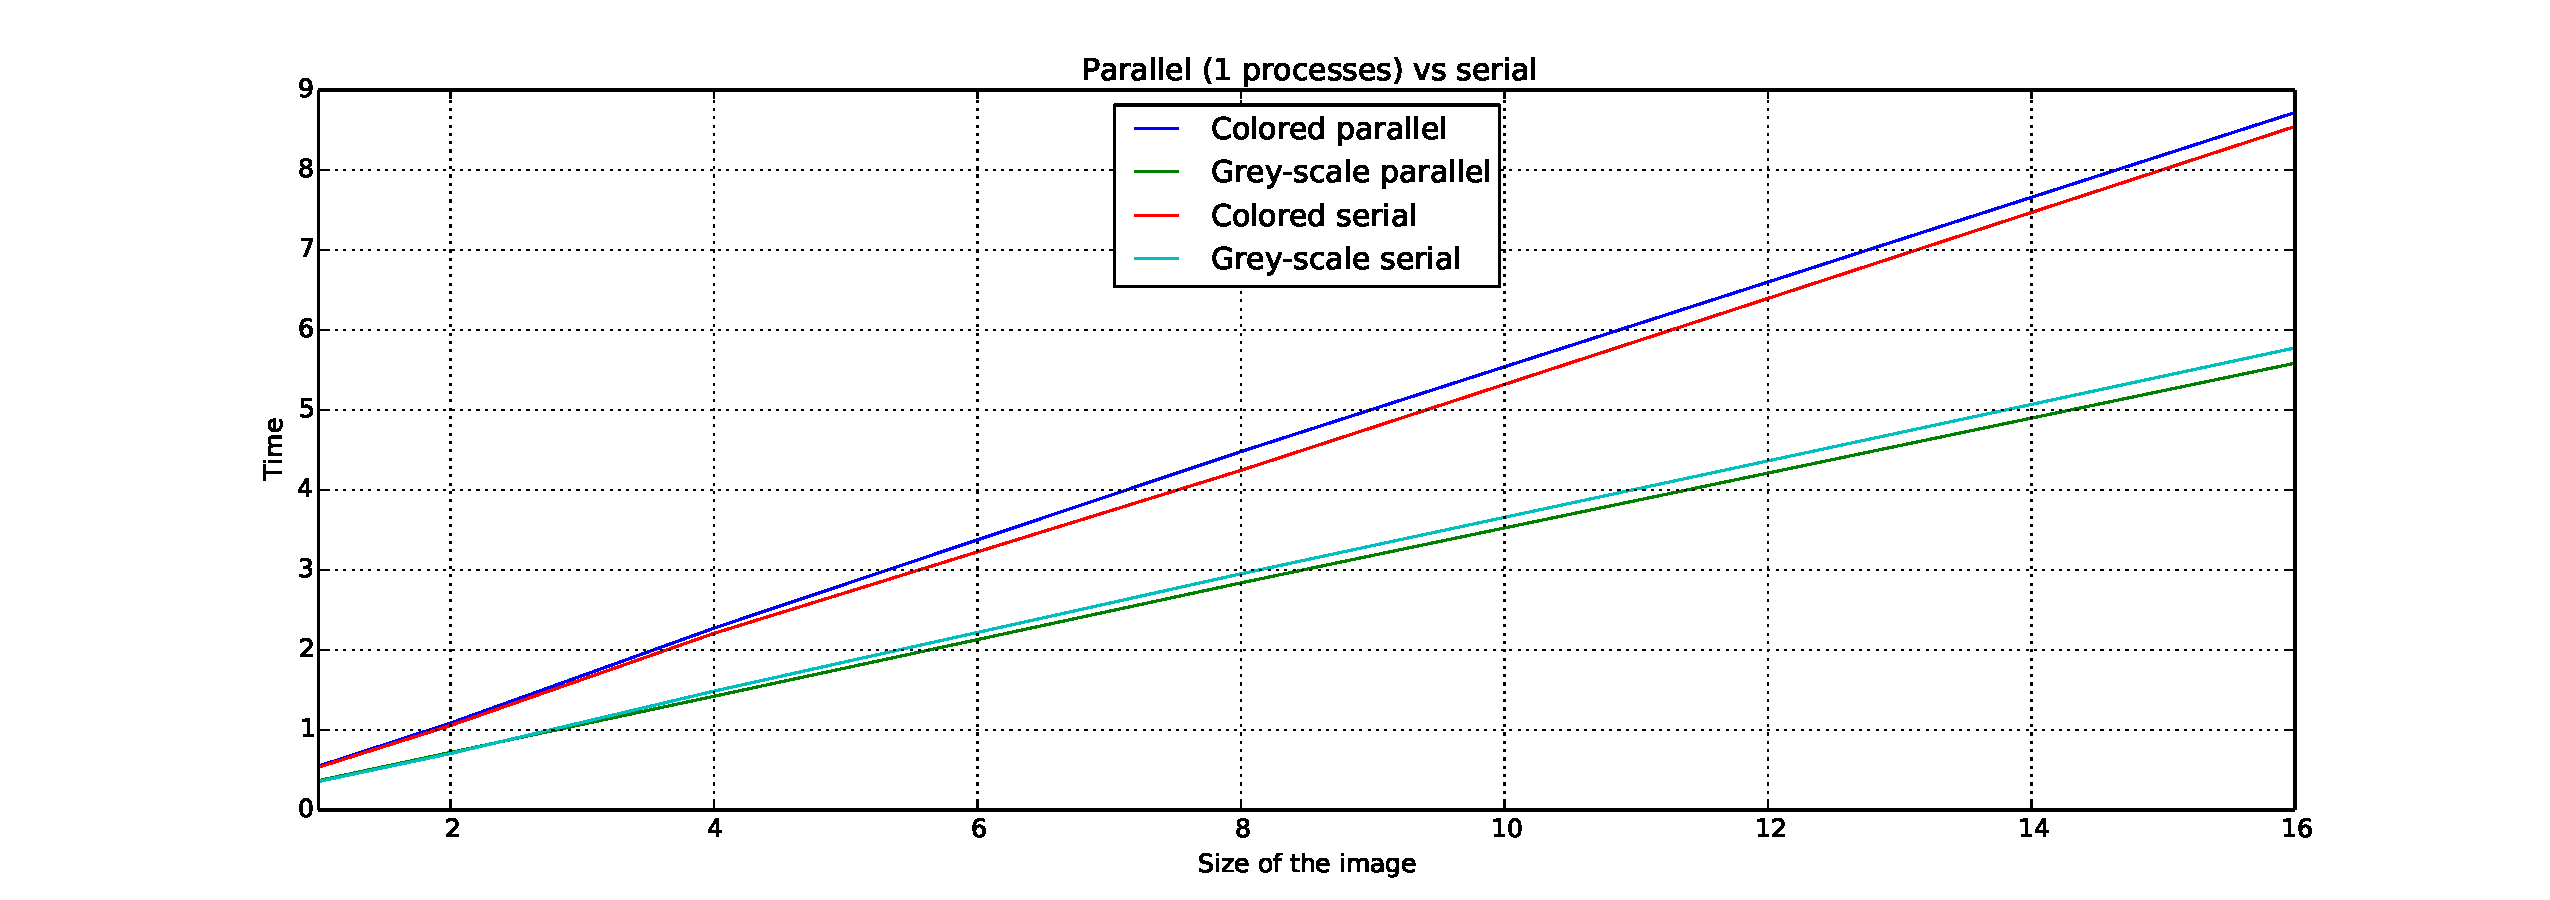
\includegraphics[width=\textwidth]{comp-1.pdf}
    \caption{Comparing serial with parallel (1 processes)}
\end{figure}

\begin{figure}[h]
    \centering
    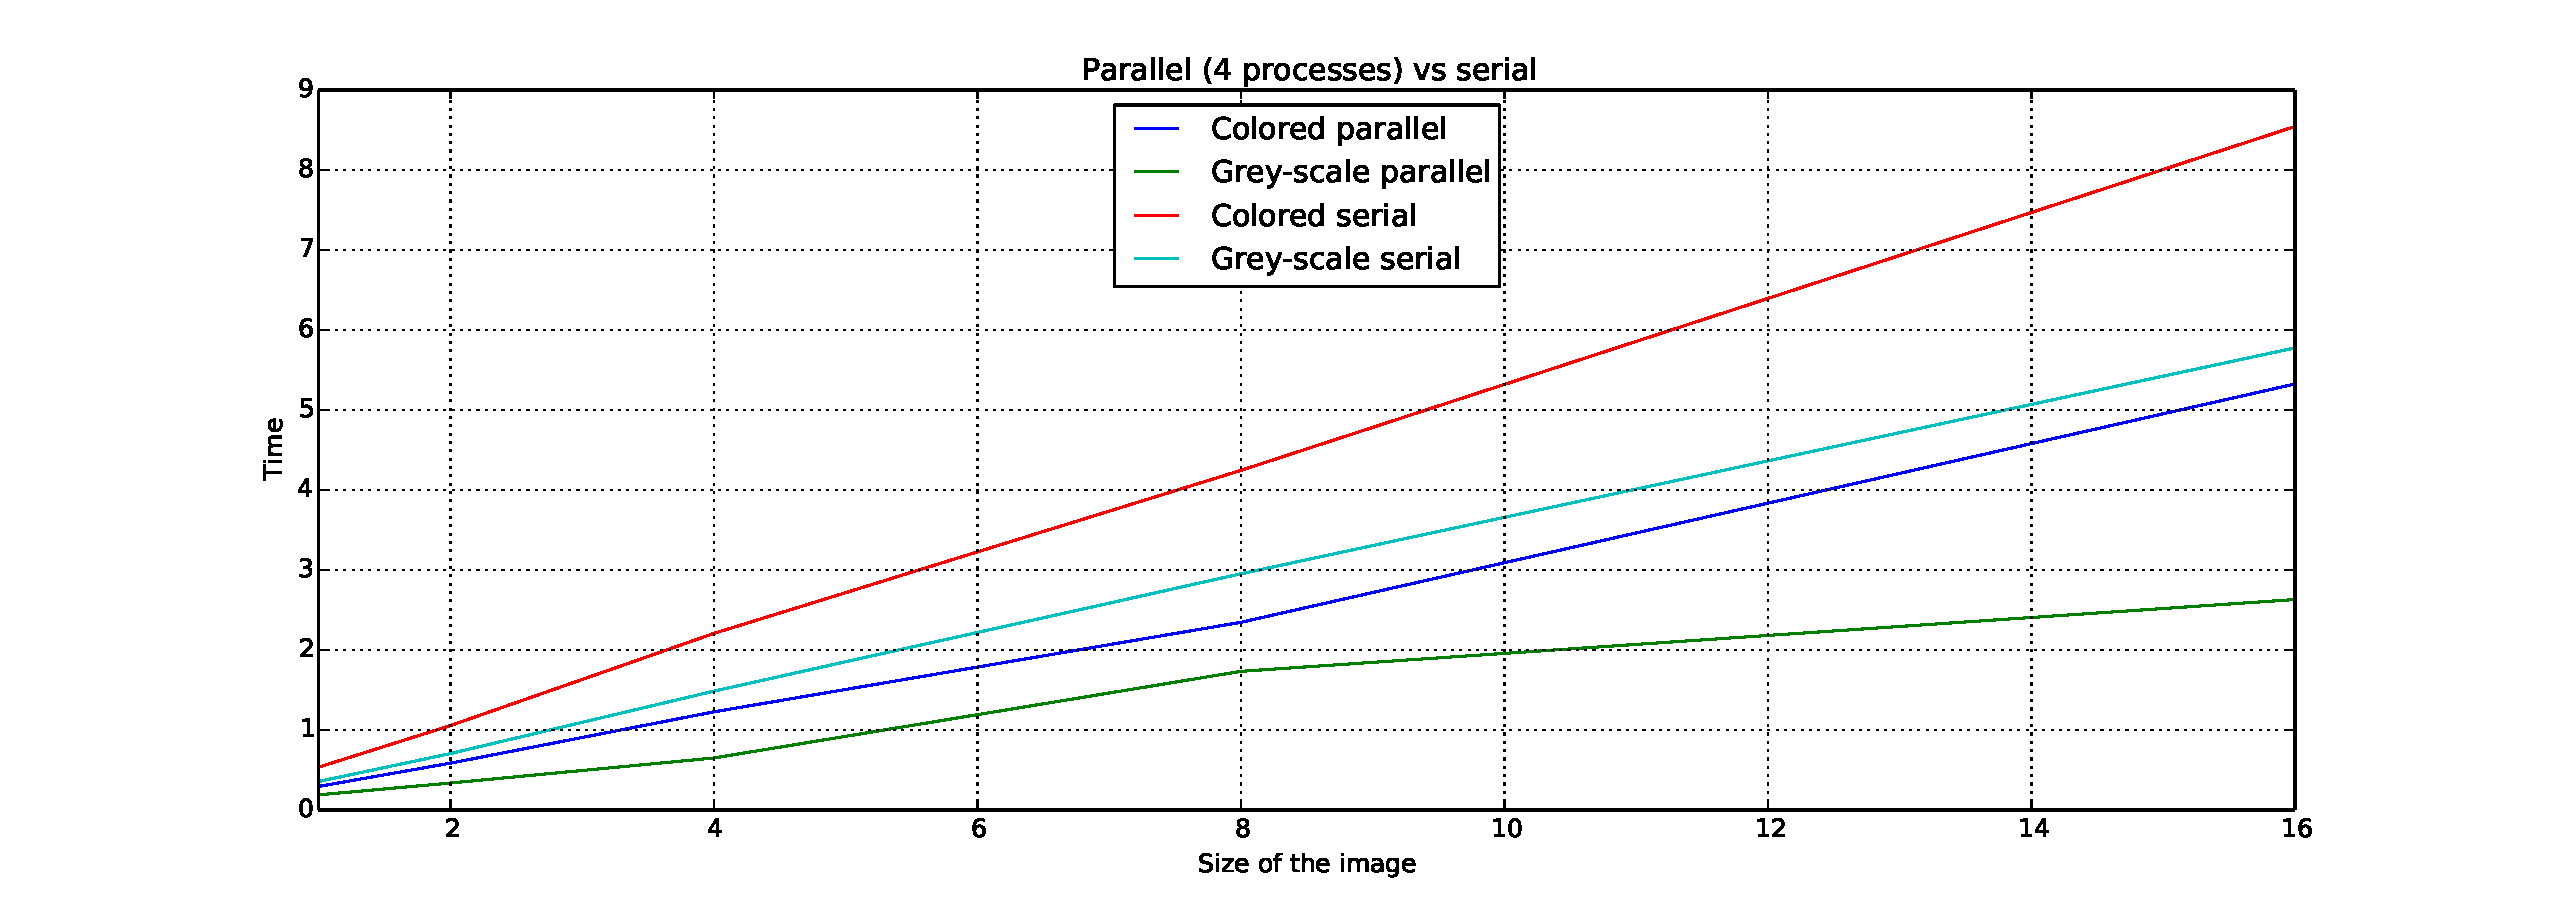
\includegraphics[width=\textwidth]{comp-4.pdf}
    \caption{Comparing serial with parallel (4 processes)}
\end{figure}

\begin{figure}[h]
    \centering
    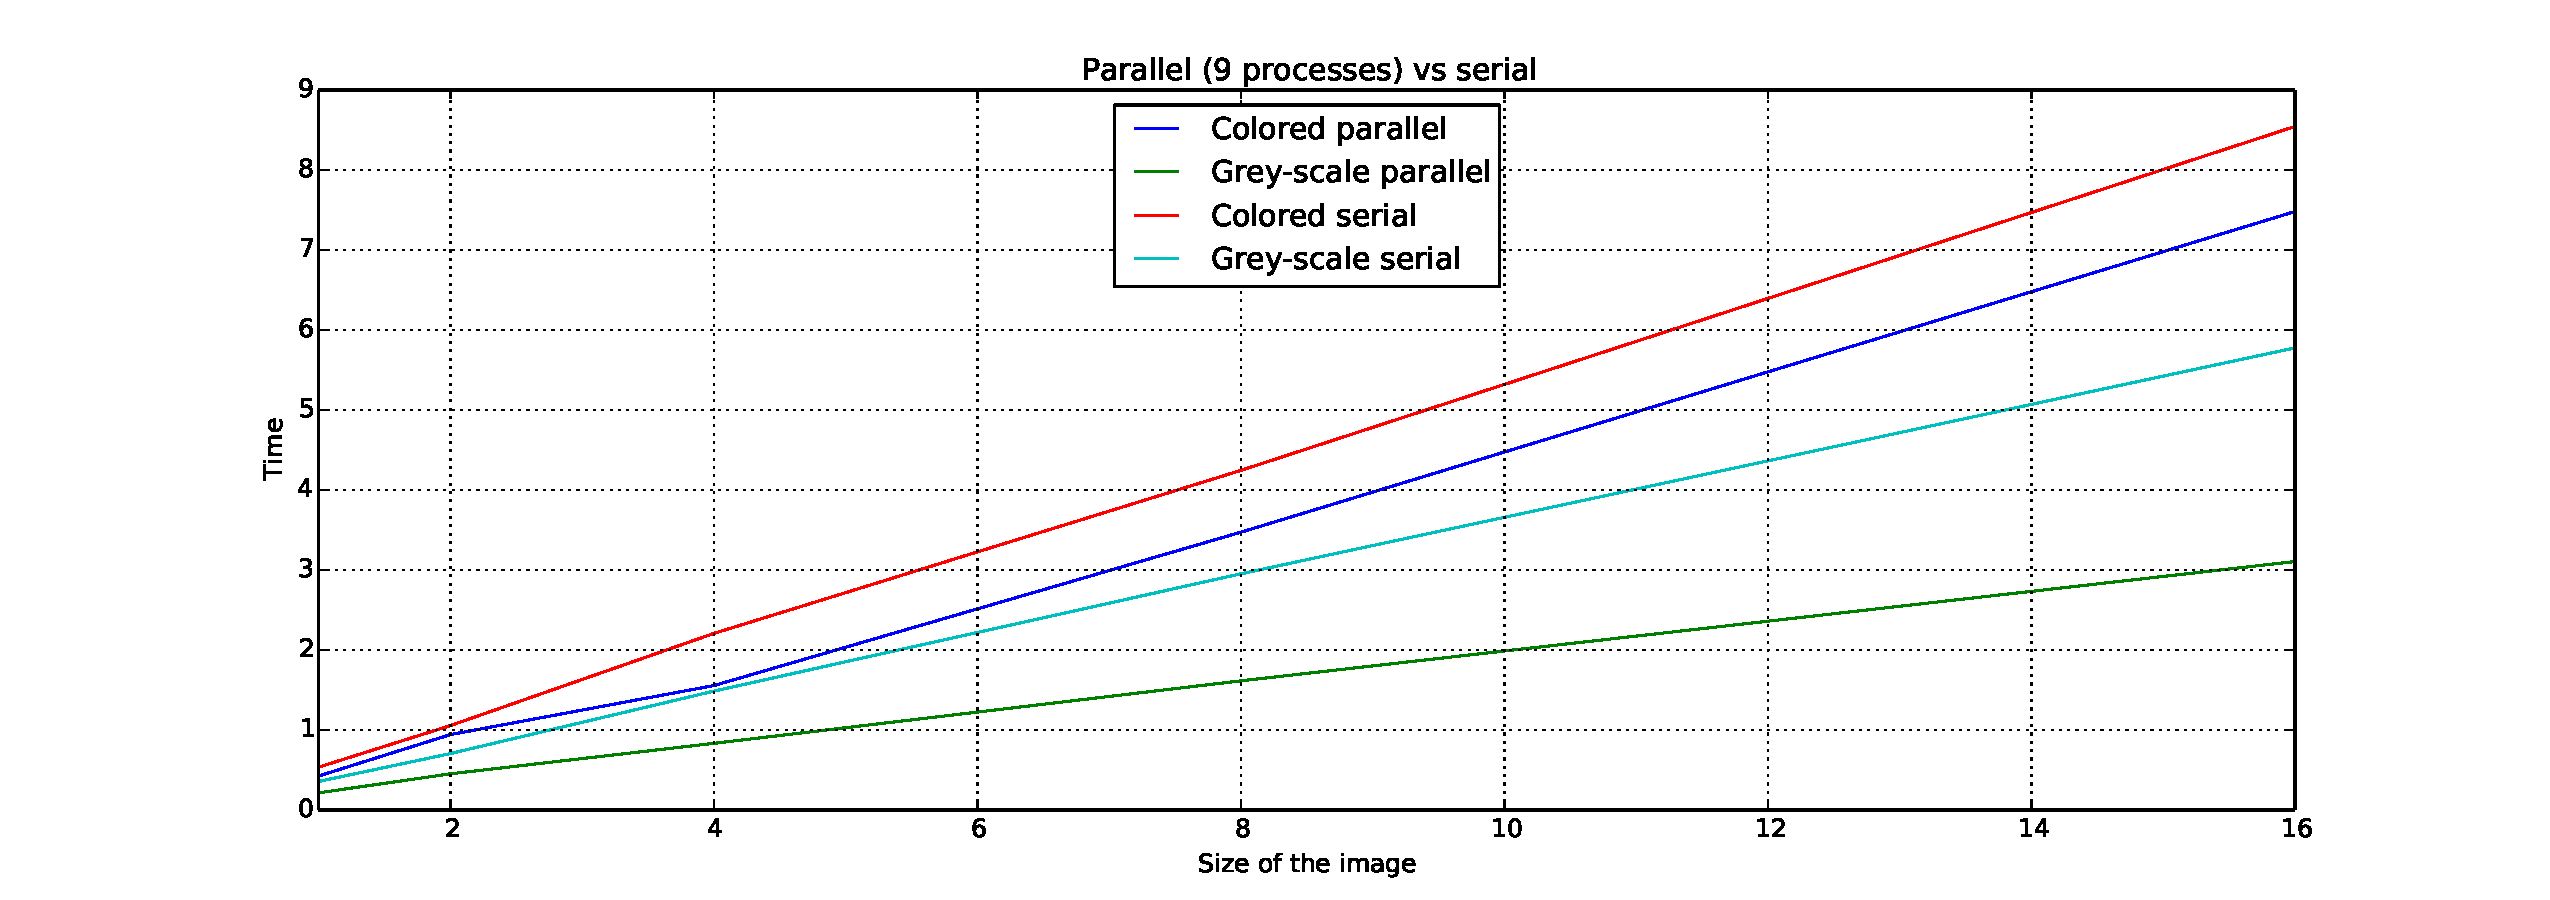
\includegraphics[width=\textwidth]{comp-9.pdf}
    \caption{Comparing serial with parallel (9 processes)}
\end{figure}

\begin{figure}[h]
    \centering
    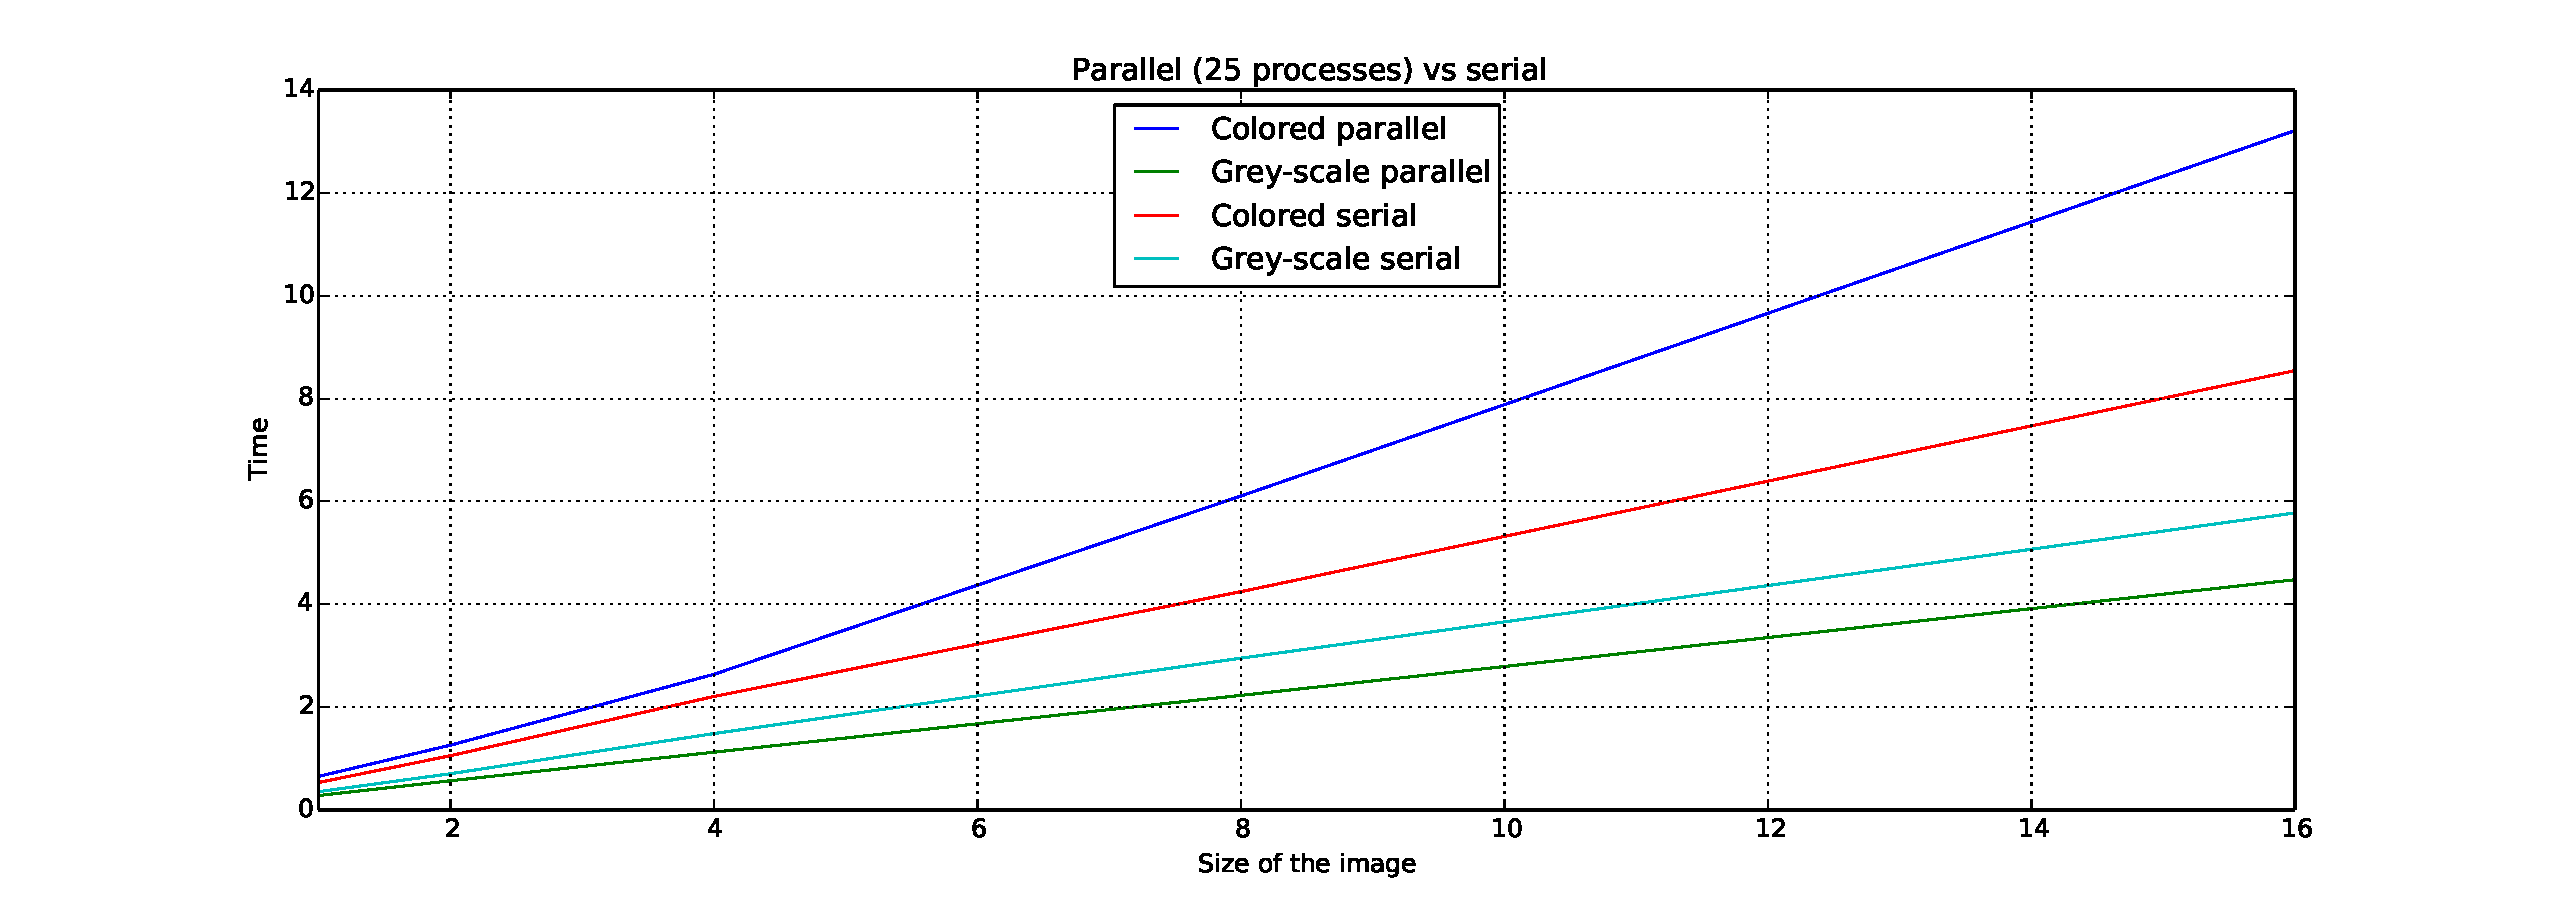
\includegraphics[width=\textwidth]{comp-25.pdf}
    \caption{Comparing serial with parallel (25 processes)}
\end{figure}

\begin{figure}[h]
    \centering
    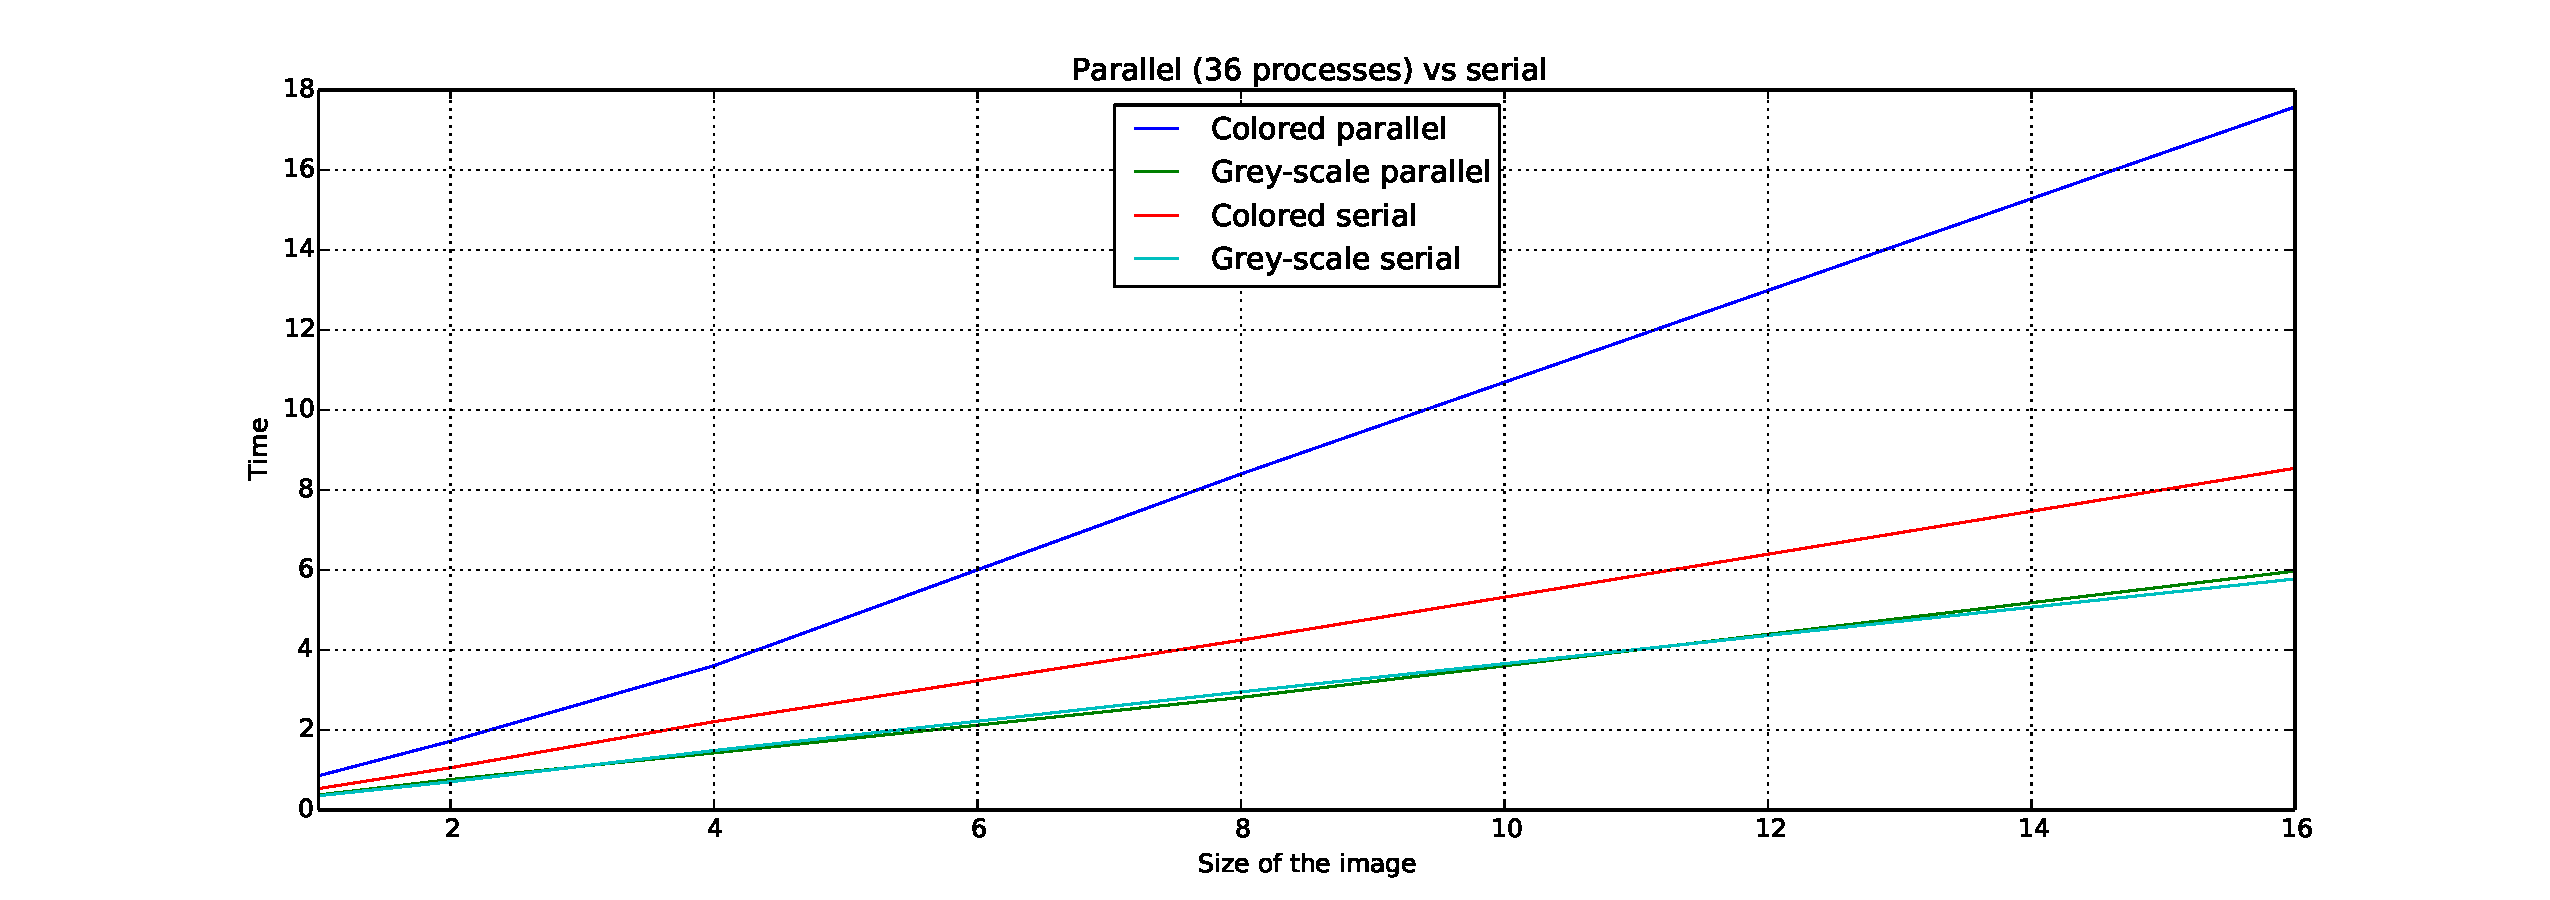
\includegraphics[width=\textwidth]{comp-36.pdf}
    \caption{Comparing serial with parallel (36 processes)}
\end{figure}

In the following figures, we compare the parallel and serial timings of
different problem sizes. Seems that above 9 processes the parallel
implementation becomes slower. Additionally, I include figures that show how
the number of processes change the timings for different problem sizes.

\begin{figure}[h]
    \centering
    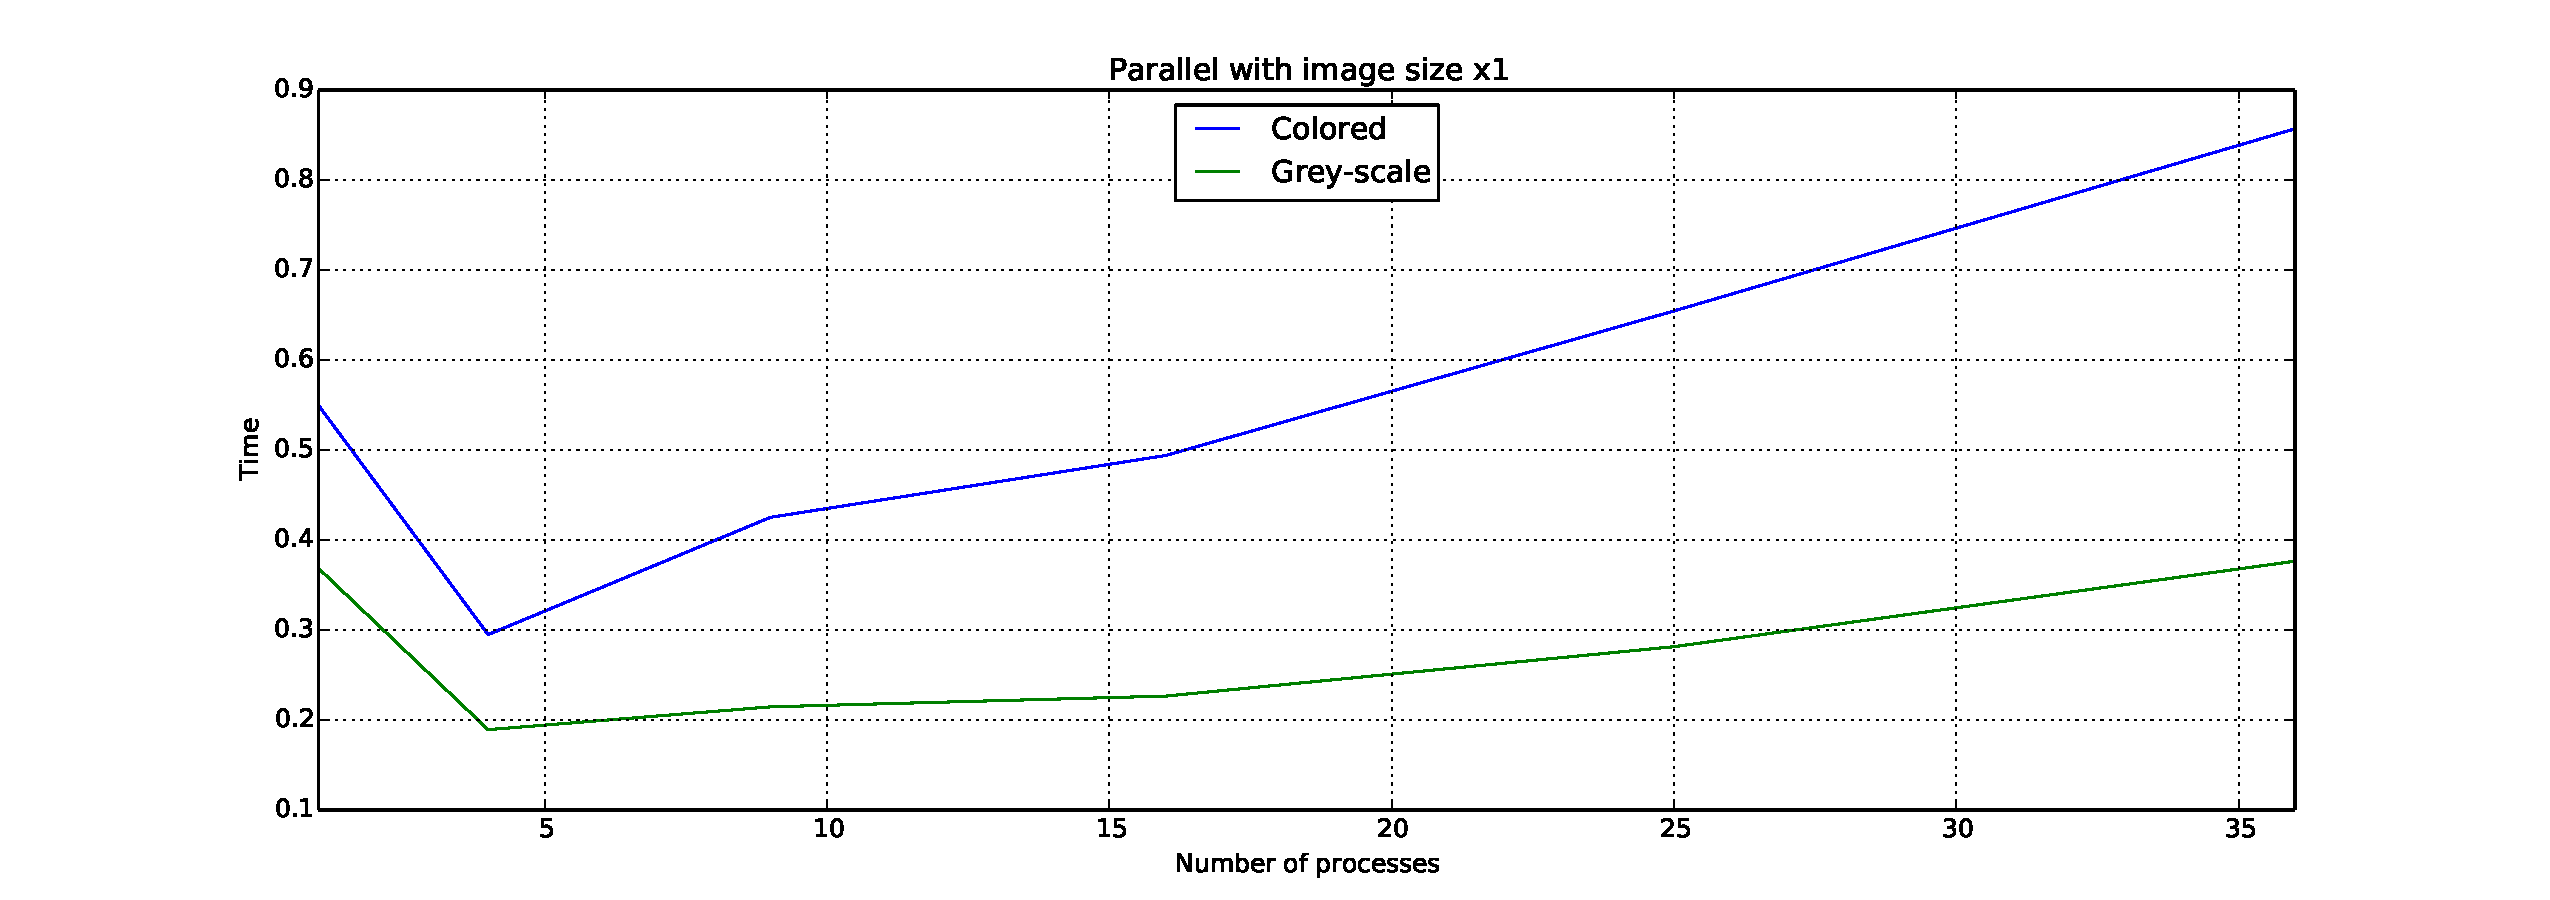
\includegraphics[width=\textwidth]{parallel-1.pdf}
    \caption{Comparing number of processes values for image size 1x}
\end{figure}

\begin{figure}[h]
    \centering
    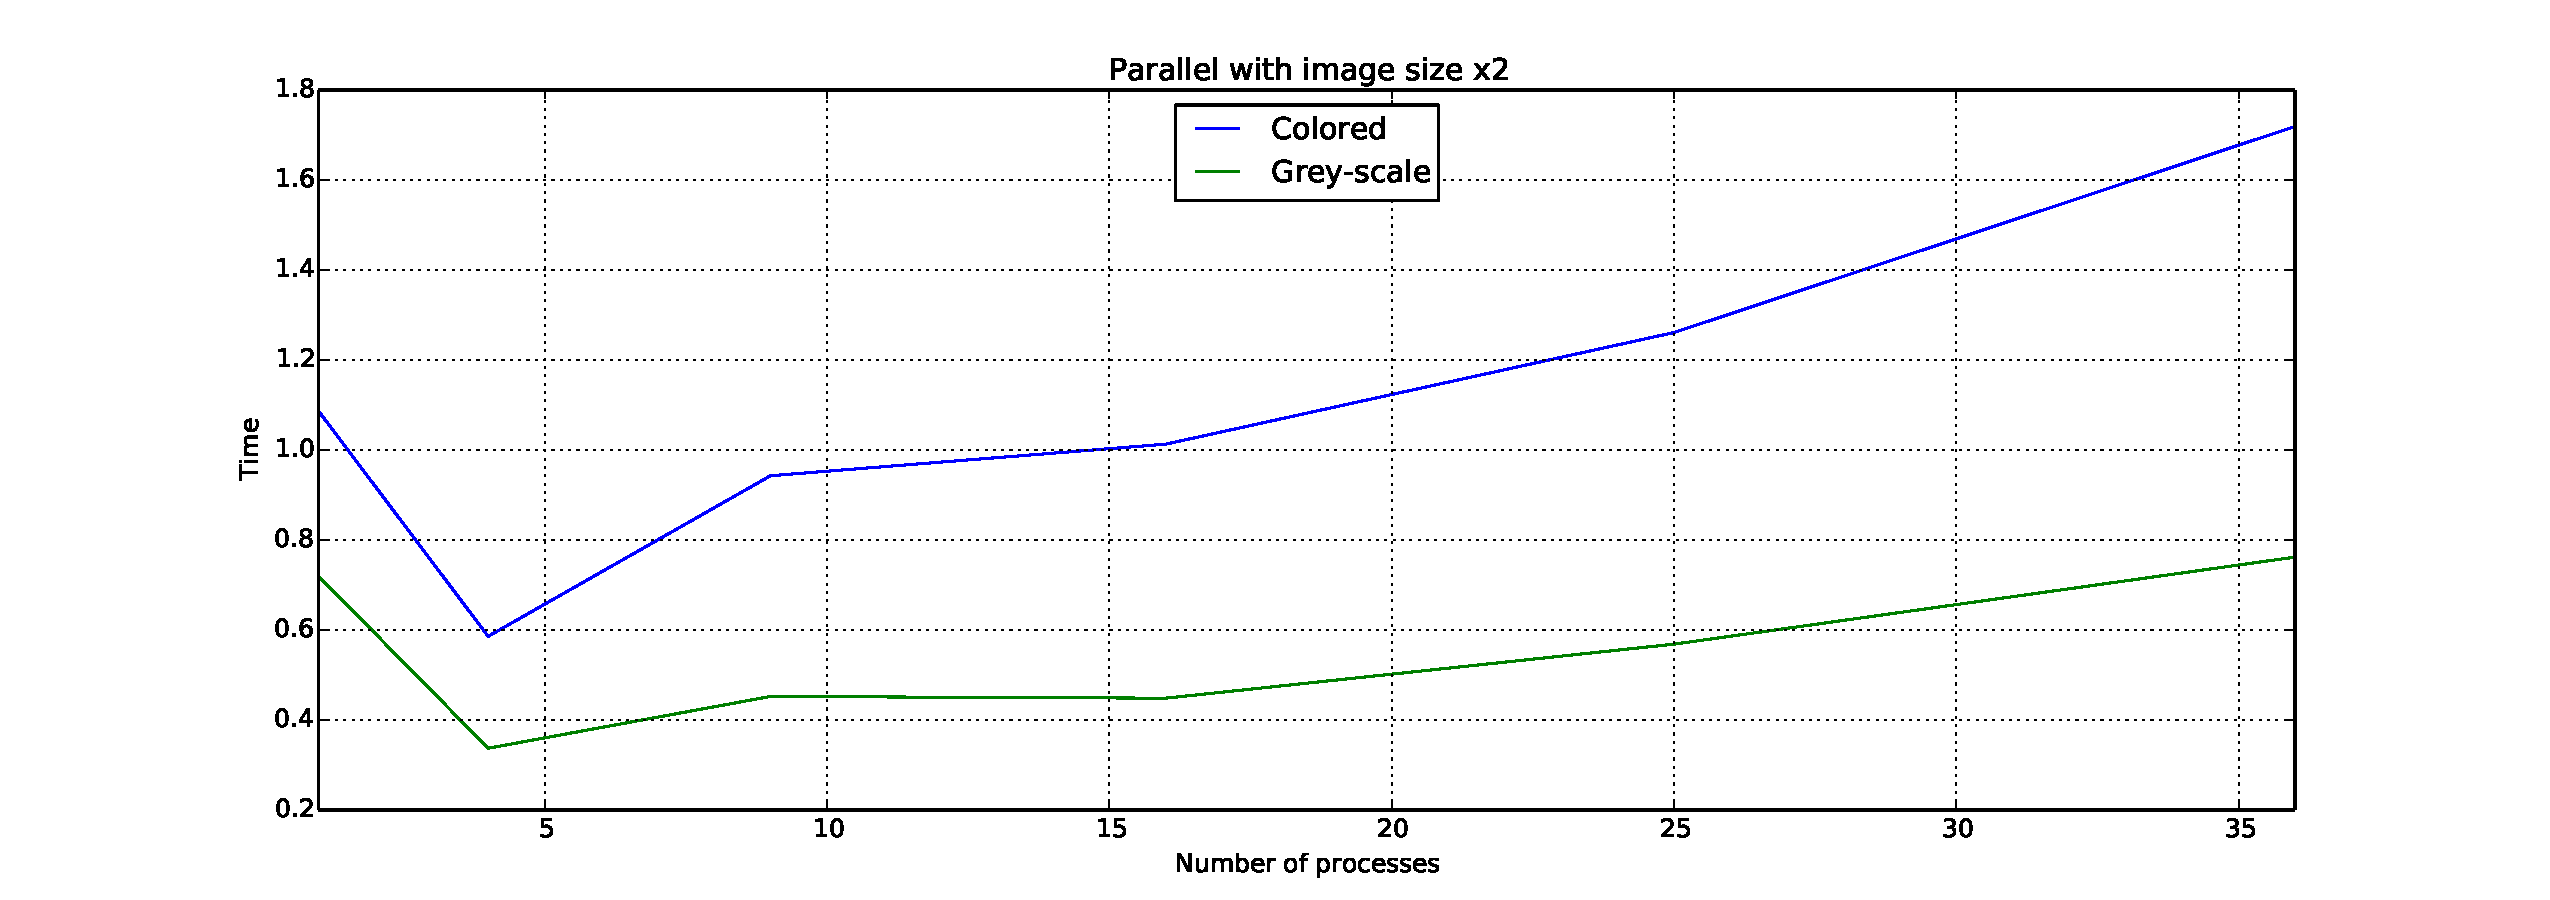
\includegraphics[width=\textwidth]{parallel-2.pdf}
    \caption{Comparing number of processes values for image size 2x}
\end{figure}

\begin{figure}[h]
    \centering
    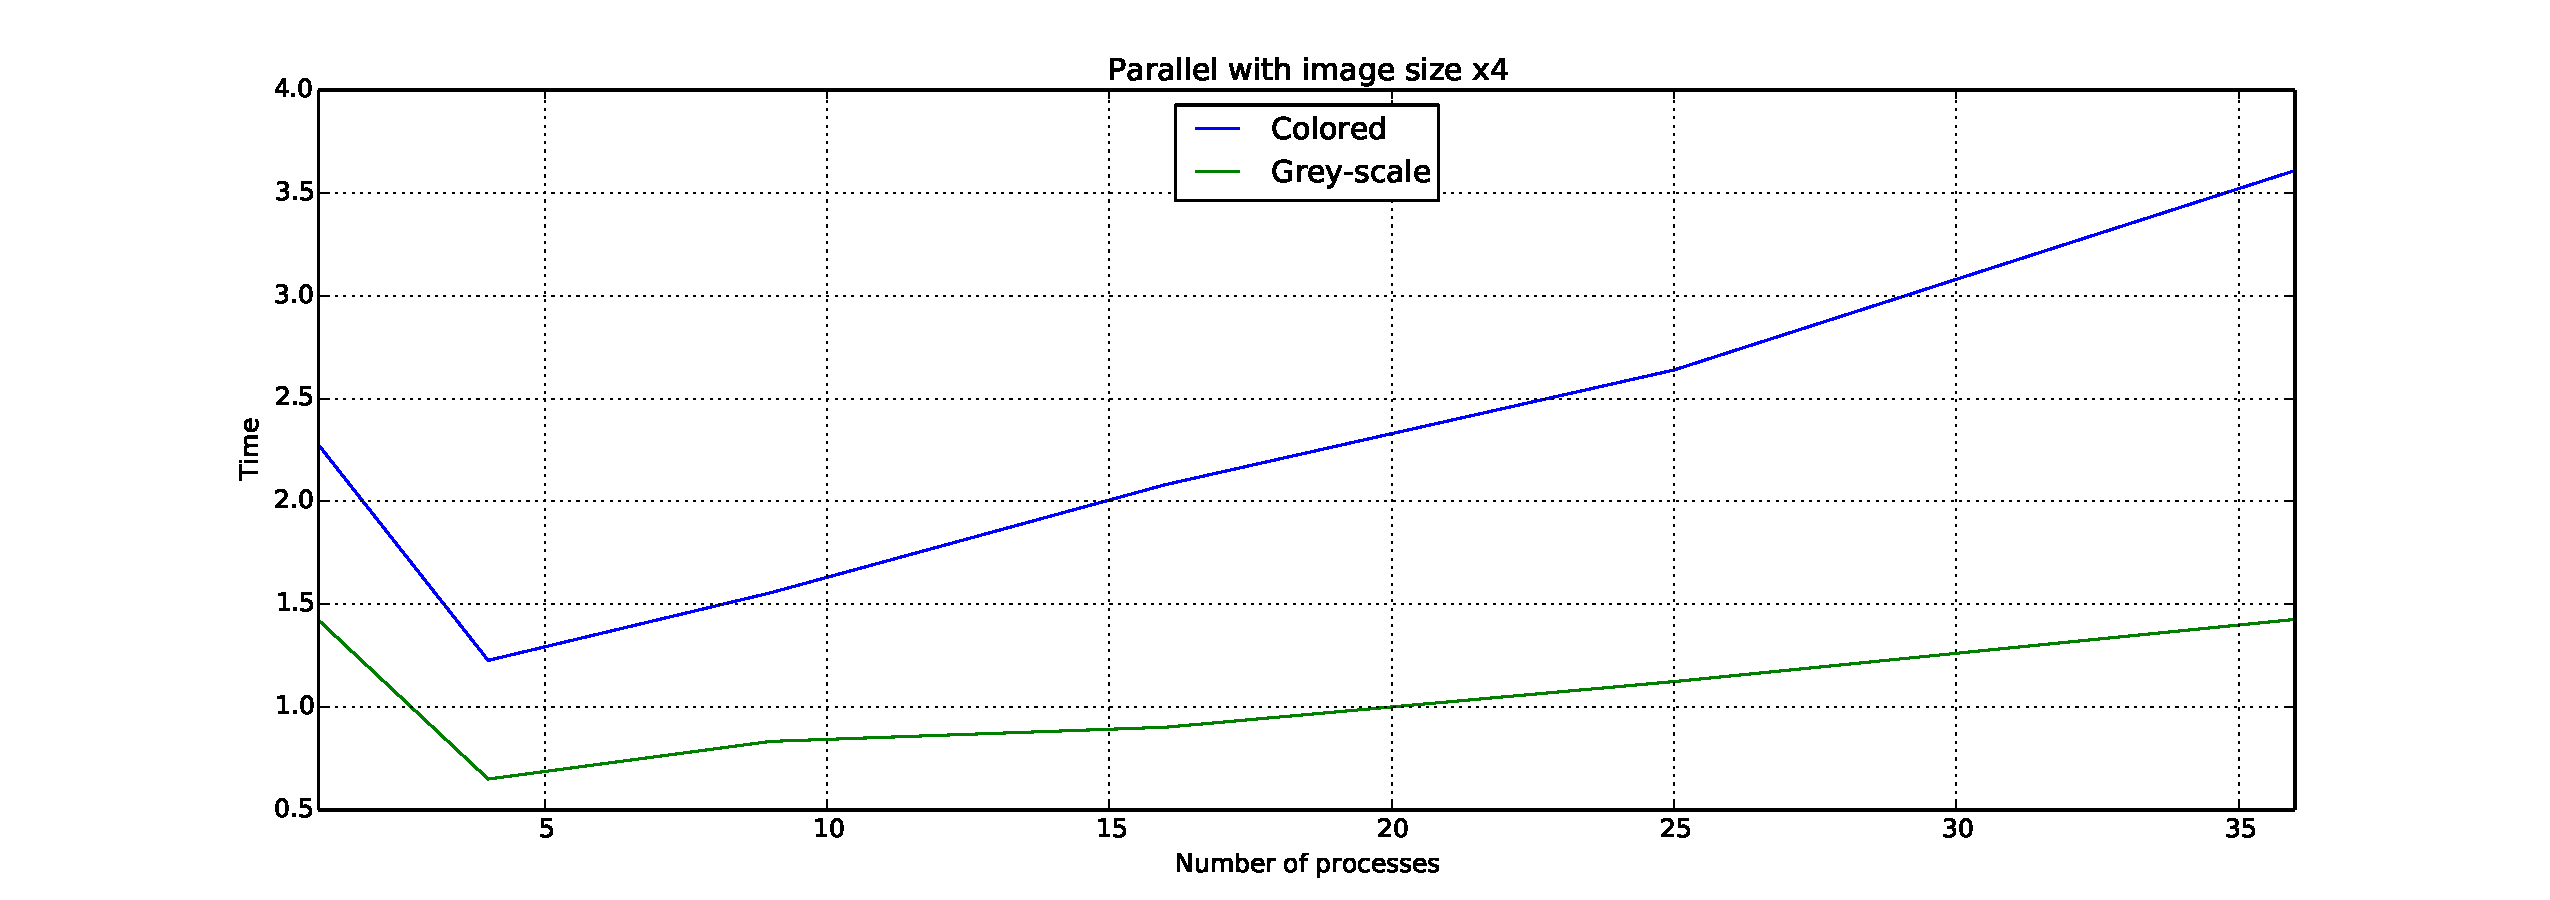
\includegraphics[width=\textwidth]{parallel-4.pdf}
    \caption{Comparing number of processes values for image size 4x}
\end{figure}

\begin{figure}[h]
    \centering
    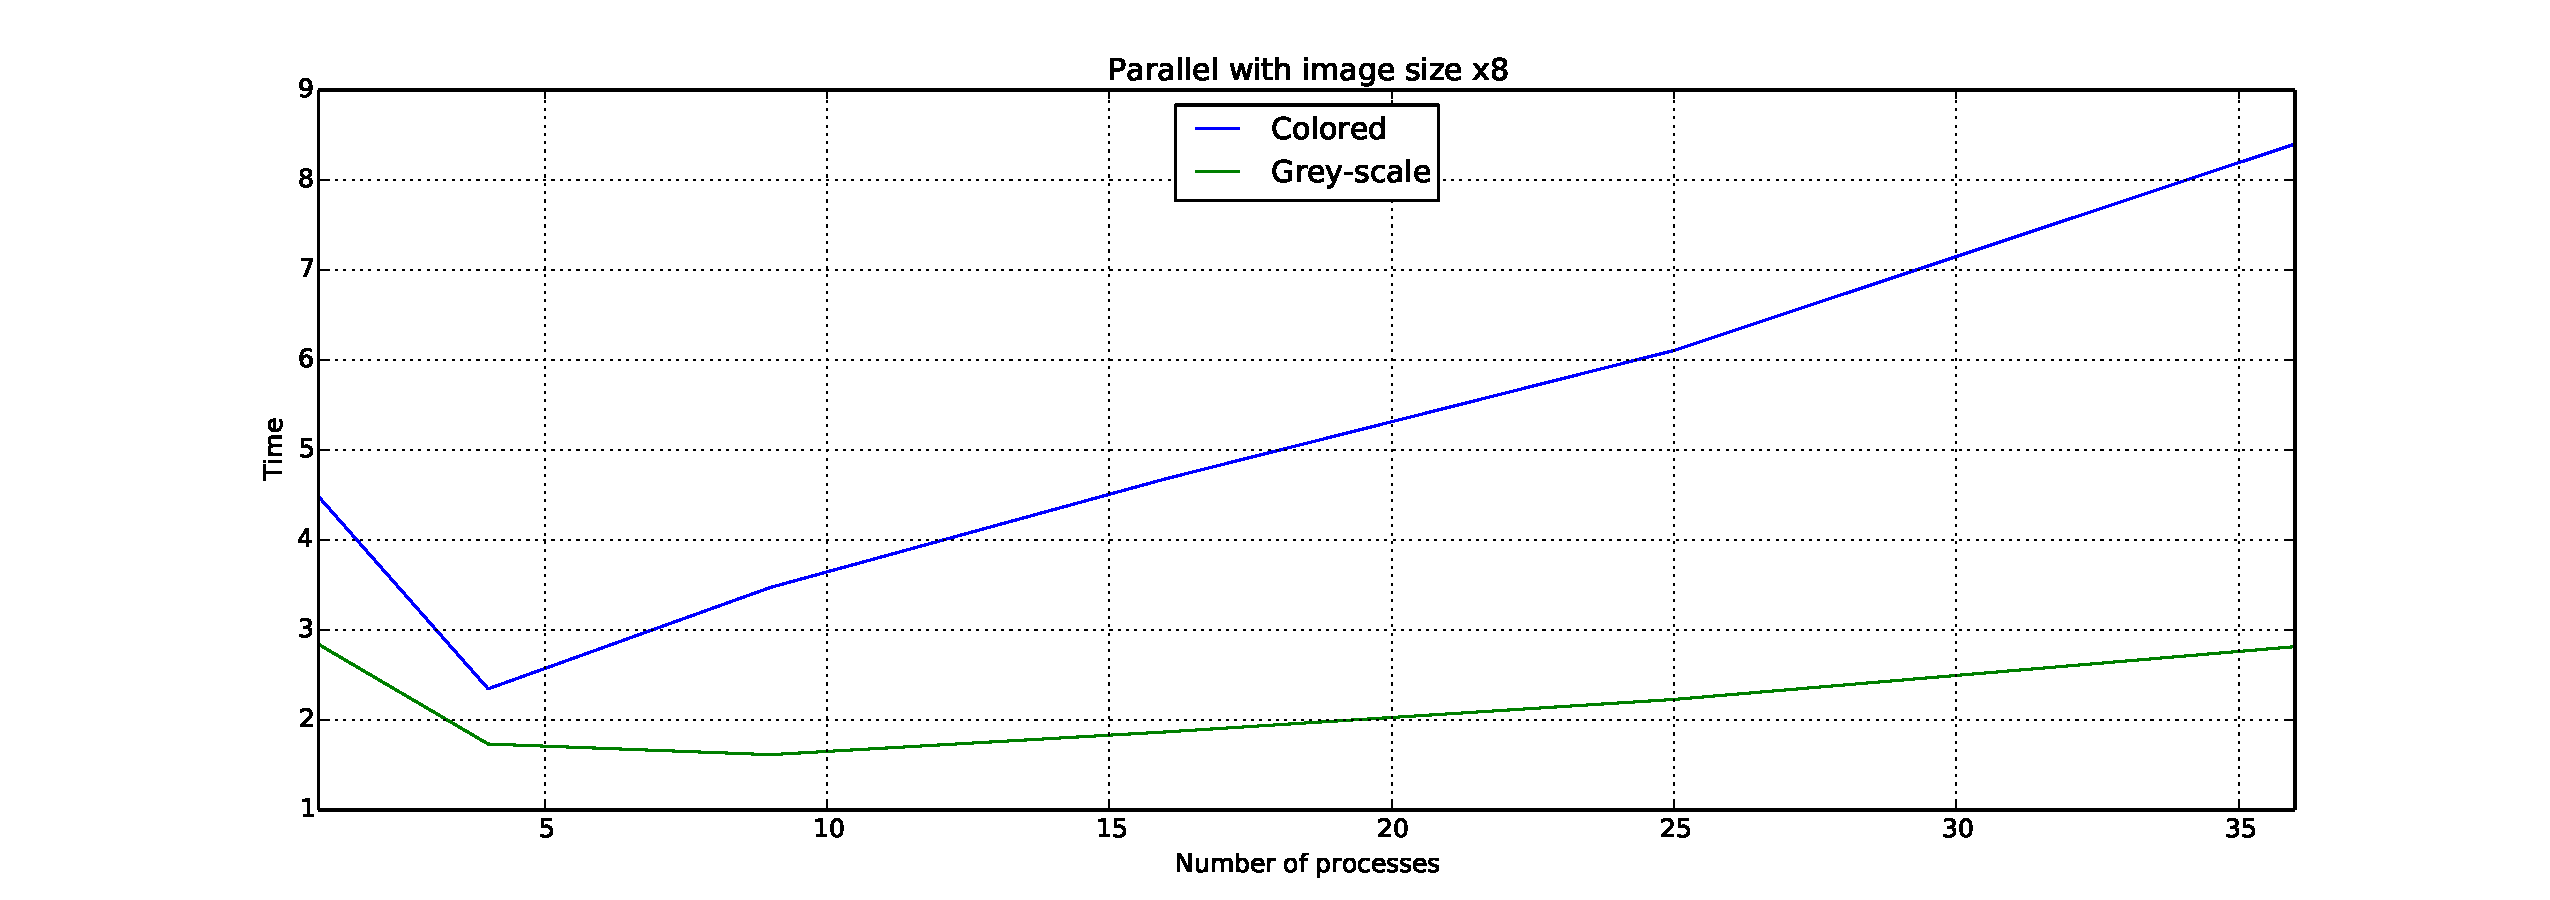
\includegraphics[width=\textwidth]{parallel-8.pdf}
    \caption{Comparing number of processes values for image size 8x}
\end{figure}

\begin{figure}[h]
    \centering
    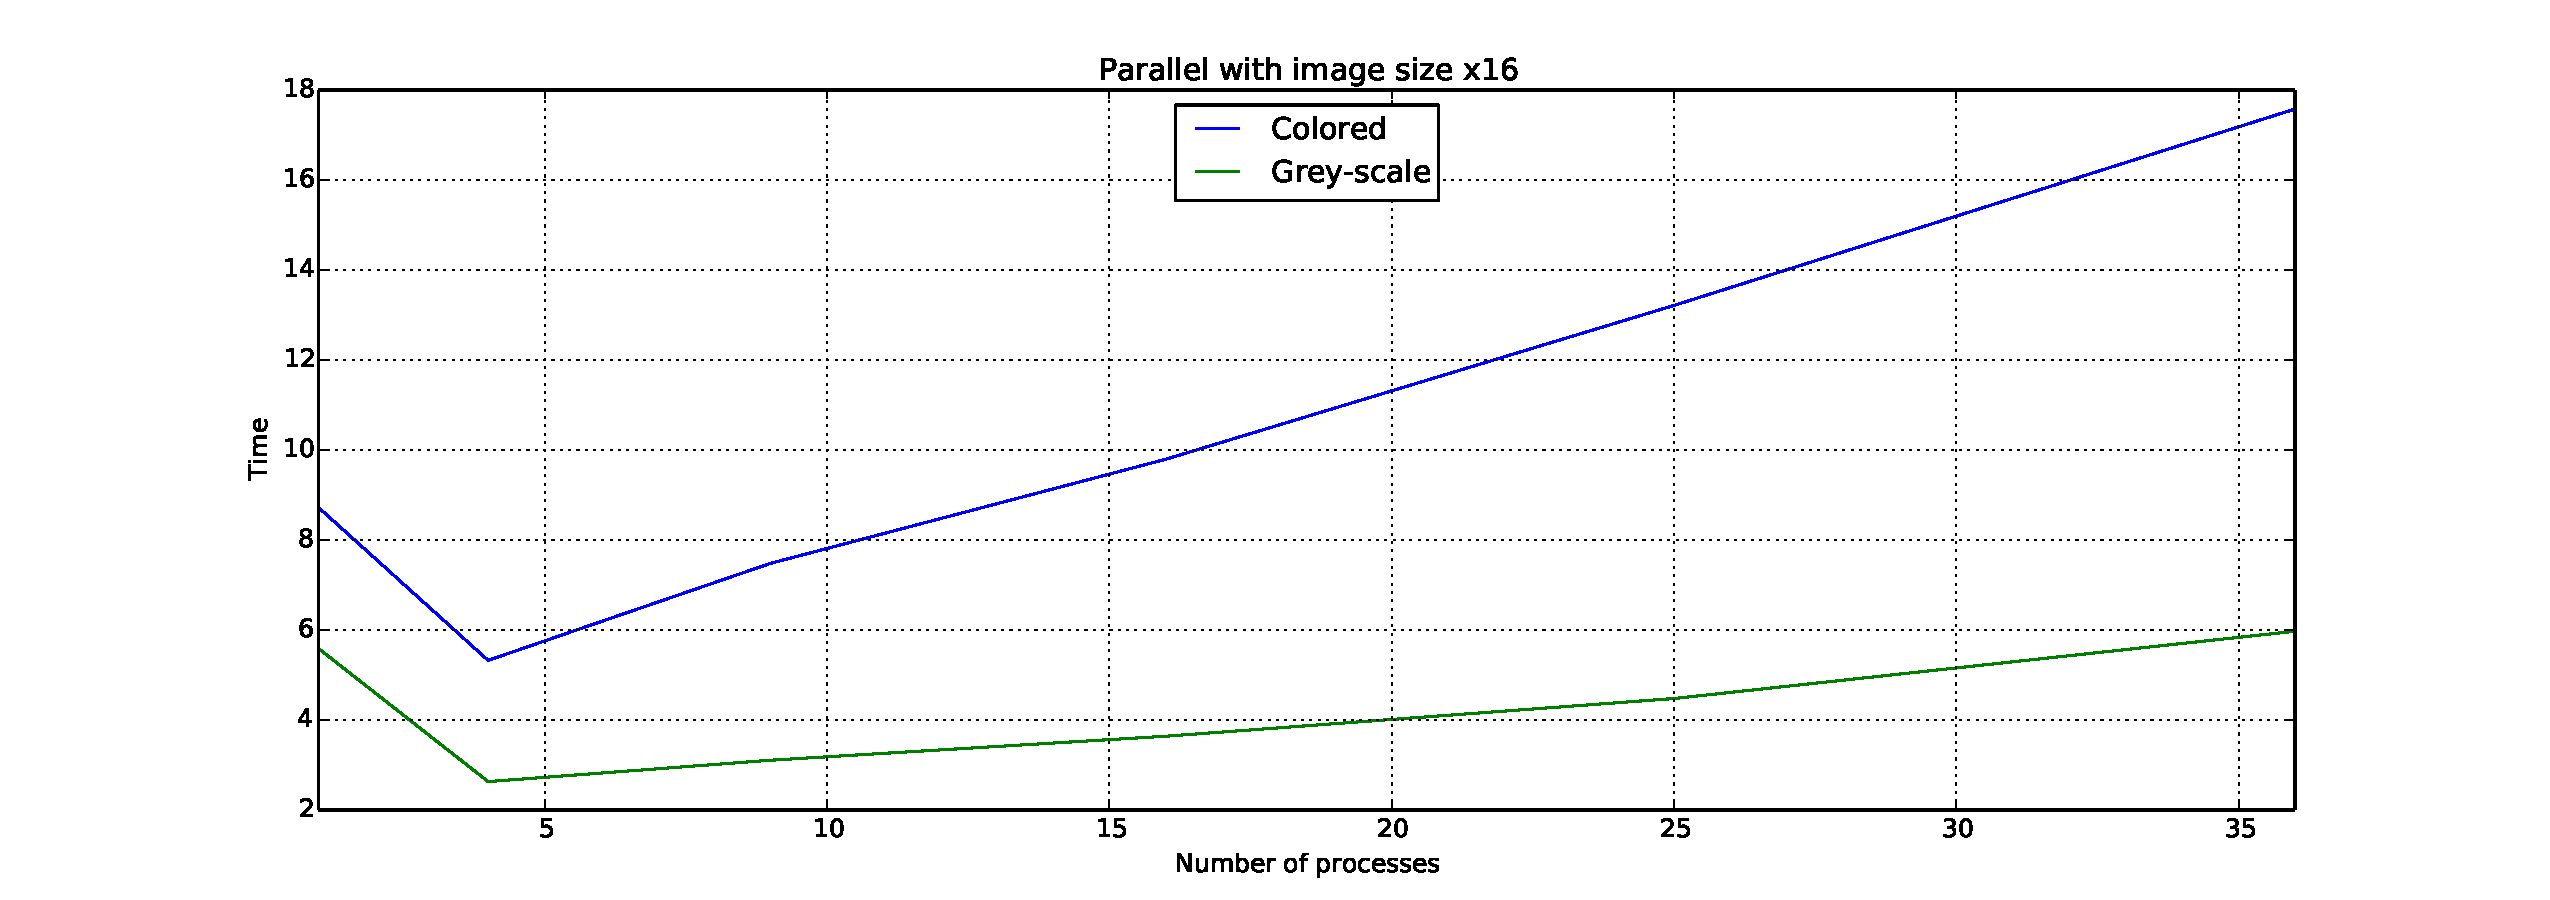
\includegraphics[width=\textwidth]{parallel-16.pdf}
    \caption{Comparing number of processes values for image size 16x}
\end{figure}

%%%%%%%%%%%%%%%%%%%%%%%%%%%%%%%%%%%%%%%%%%%%%%%%%%%%%%%%%%%%%%%%%%%%%%%%%%%%%%%%

%%%%%%%%%%%%%%%%%%%%%%%%%%%%%%%%%%%%%%%%%%%%%%%%%%%%%%%%%%%%%%%%%%%%%%%%%%%%%%%%
% Possible extensions
%%%%%%%%%%%%%%%%%%%%%%%%%%%%%%%%%%%%%%%%%%%%%%%%%%%%%%%%%%%%%%%%%%%%%%%%%%%%%%%%

\section{Possible extensions}

There are a several things that could be improved in the current
implementation.

The \texttt{struct image\_t} memory usage, especially when it comes to the
worker memory footprint:
\begin{itemize}
    \item The type uses memory to maintain a \texttt{rows} list for easier
        access to the image rows. This is certainly redundant.
    \item In the case of the worker input image, it is known that
        only a small fragment of the image is actually filled. The rest
        is not used. Hence something could be done here to reduce image's
        memory footprint for the worker process.
\end{itemize}

The communication scheme can be improved aiming for the following:
\begin{itemize}
    \item More fair load balancing between root and worker processes. A
        tree-structured communication scheme could be used instead.
    \item Ability to ran the process several times without having to
        resend the whole image.
\end{itemize}

%%%%%%%%%%%%%%%%%%%%%%%%%%%%%%%%%%%%%%%%%%%%%%%%%%%%%%%%%%%%%%%%%%%%%%%%%%%%%%%%

\end{document}
